% !TEX root = ../../main.tex

% Reset graphics to the current folder
\graphicspath{ {\thisch/figures/} }

\chapter{Appendix for \autoref{calo}}%
\label{appx:calo}

\begin{figure}[H]
    \centering
    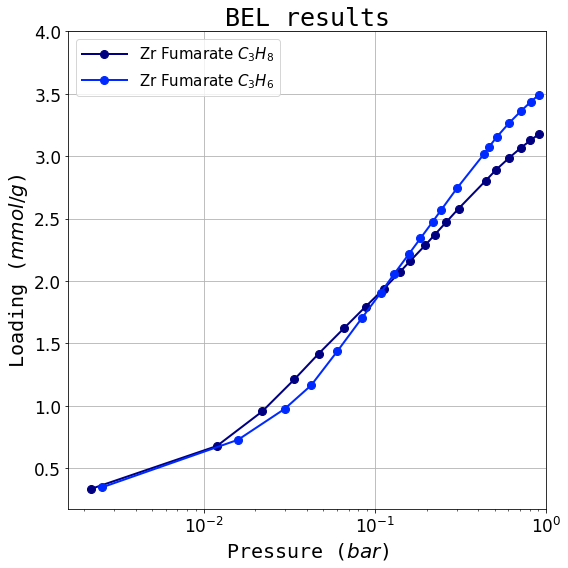
\includegraphics[width=0.6\linewidth]{zrfum/zrfum-bel}
    \caption{
        Propane and propylene isotherms recorded on Zr Fumarate
        in a commercial volumetric apparatus (BEL Mini). 
    }\label{appx:calo:fgr:zrfum-bel}
\end{figure}

\begin{figure}[H]
    \centering
    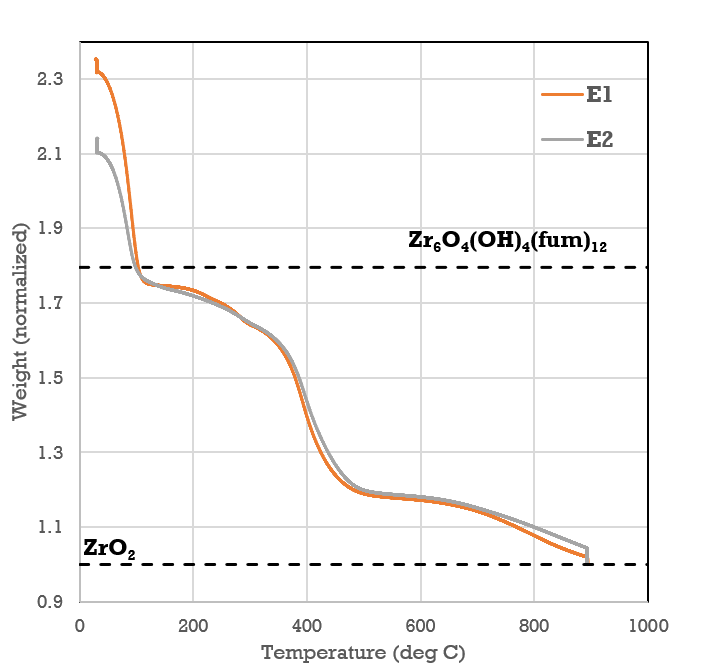
\includegraphics[width=0.6\linewidth]{zrfum/zrfum-tga}
    \caption{
        Thermogravimetric experiments highlighting the
        presence of defects in the Zr Fumarate structure.
    }\label{appx:calo:fgr:zrfum-tga}
\end{figure}

\begin{figure}[H]
    \centering
    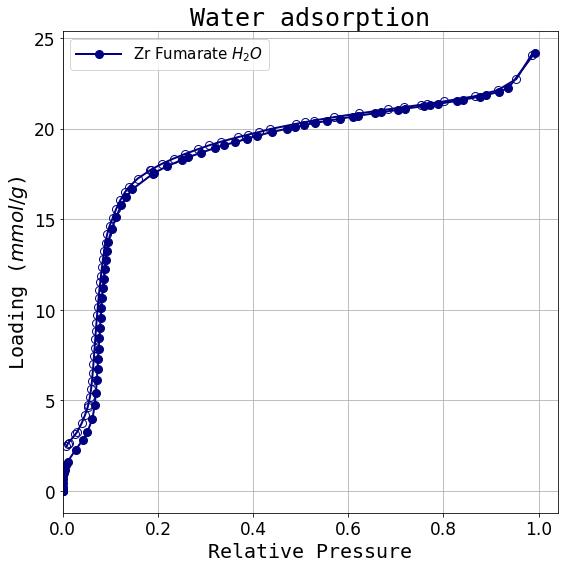
\includegraphics[width=0.6\linewidth]{zrfum/zrfum-water}
    \caption{
        Water isotherm recorded on Zr Fumarate. The 
        steep adsorption curve at below \(0.2~p/p_0\) is an 
        indication of defects in the MOF 
        structure~\cite{choiRoleStructuralDefects2018}.
    }\label{appx:calo:fgr:zrfum-water}
\end{figure}

\FloatBarrier{}
\pagebreak

\bibliographystyle{unsrtnat}
\bibliography{backmatter/biblio/bib}